\documentclass[12pt]{report}
\usepackage[margin=1in]{geometry}
\usepackage{amsmath,amsthm,amssymb}
\usepackage{graphicx}
\graphicspath{ {images/} }
 
\newcommand{\N}{\mathbb{N}}
\newcommand{\Z}{\mathbb{Z}}
\newcommand{\R}{\mathbb{R}}
\newcommand{\Indicator}{\mathds{1}}
\newcommand{\EX}{\mathbb{E}}
\newcommand{\Prob}{\mathbb{P}}

\begin{document}


\section{Minimizing the Expectations}

\subsection{The Balanced Loss Function}

To compute the balanced policy, the following equation must be minimized.

$$
	g_s(q_s^B) = \max\{l_s^B(q_s), \pi_s^B(q_s)\}
$$
where $l_s^B(q_s), \pi_s^B(q_s)$ are as they were defined previously. For general distributions, these equations can be difficult to solve. However, assuming the demand has a multivariate normal distribution, there is a closed form solution.  

\subsection{Marginal Holding Cost $l_s^B(q_s)$}

Computing $l_s^B(q_s)$ in the general case requires the computation of a $T - s$ dimensional integral. Traditional quadrature algorithms have exponential complexity in dimensions, making such an integral unreasonable to compute. However, some conditions allow it to be reduced to $T-s$ integrals of fewer dimensions. Letting $\Phi$ be the (generally multivariate) distribution of forecast $f_s$: 
\begin{alignat*}{1}
	l_s^B(q_s) &= \EX [H_s^B(q_s) \; | \; f_s] \\
        &= \EX \bigg\{\sum_{j=s}^T h_j\bigg[q_s - \bigg(\sum_{i=s}^j u_i - X_s\bigg)^+\bigg]^+  \; | \; f_s \bigg\} \\
		&= \int_{u_s}^{\infty} \int_{u_{(s+1)}}^{\infty}\dots \int_{u_T}^{\infty}\sum_{j=s}^T h_j\bigg[q_s - \bigg(\sum_{i=s}^j u_i - X_s\bigg)^+\bigg]^+ d\Phi(u_s, u_{s+1}, \dots u_T)\\
	   &= \sum_{j=s}^T \int_{u_s}^{\infty} \int_{u_{(s+1)}}^{\infty}\dots \int_{u_j}^{\infty} h_j\bigg[q_s - \bigg(\sum_{i=s}^j u_i - X_s\bigg)^+\bigg]^+ d\Phi(u_s, u_{s+1}, \dots u_T)
\end{alignat*}
If the conditions allow for $D_{[s, j]} = \sum_{i=s}^j D_s$ to be expressed as a single variate distribution $\Phi_{[s, j]}$, then $l_s^B(q_s)$ can be expressed as $T - s$ integrals in one dimension:
\begin{equation}
	l_s^B(q_s) = \sum_{j=s}^T \int_{u_j=X_s}^{X_s + q_s} h_j\bigg(q_s + X_s - u_j \bigg) d\Phi_{[s, j]}(u_j)
\end{equation}
Under the same conditions, $\frac{d}{d q_s} l_s^B(q_s)$ can be expressed:
\begin{equation}
	\frac{d}{d q_s} l_s^B(q_s) =  \sum_{j=s}^T h_j (\Phi_{[s, j]}(X_s + q_s) - \Phi_{[s, j]}(X_s))
\end{equation}
This condition would hold for a series of independent random variables, as well as the summation across the dimensions of a multivariate normal distribution. 


\subsection{Myopic Penalty Function $\pi_s^B(q_s)$}

$\pi_s^B(q_s)$ is a more manageable integral.
\begin{alignat}{1}
	\pi_s^B(q_s) &= \EX [\Pi_t^B(q_s) \; | \; f_s] \nonumber \\
		&= \EX \bigg\{ p_s [D_s - (X_s^B + q_s)]^+  \; | \; f_s \bigg\} \nonumber \\
		&= \int_{u_s=({X_s^B + q_s})}^{\infty} p_s (u_s - X_s^B - q_s) d\Phi_s(u_s) \\
	\frac{d}{d q_s} \pi_s^B(q_s) &=  - \int_{u_s=({X_s^B + q_s})}^{\infty} p_s d\Phi_s(u_s) \nonumber \\
		&= - p_s (1 - \Phi_s(X_s^B + q_s)) 
\end{alignat}

\subsubsection{Loss Function}

As an informal validation, the loss function was computed exactly, and using simulated results with 100 replicates. An arbitrary scenario was picked for this task. The results are plotted below:

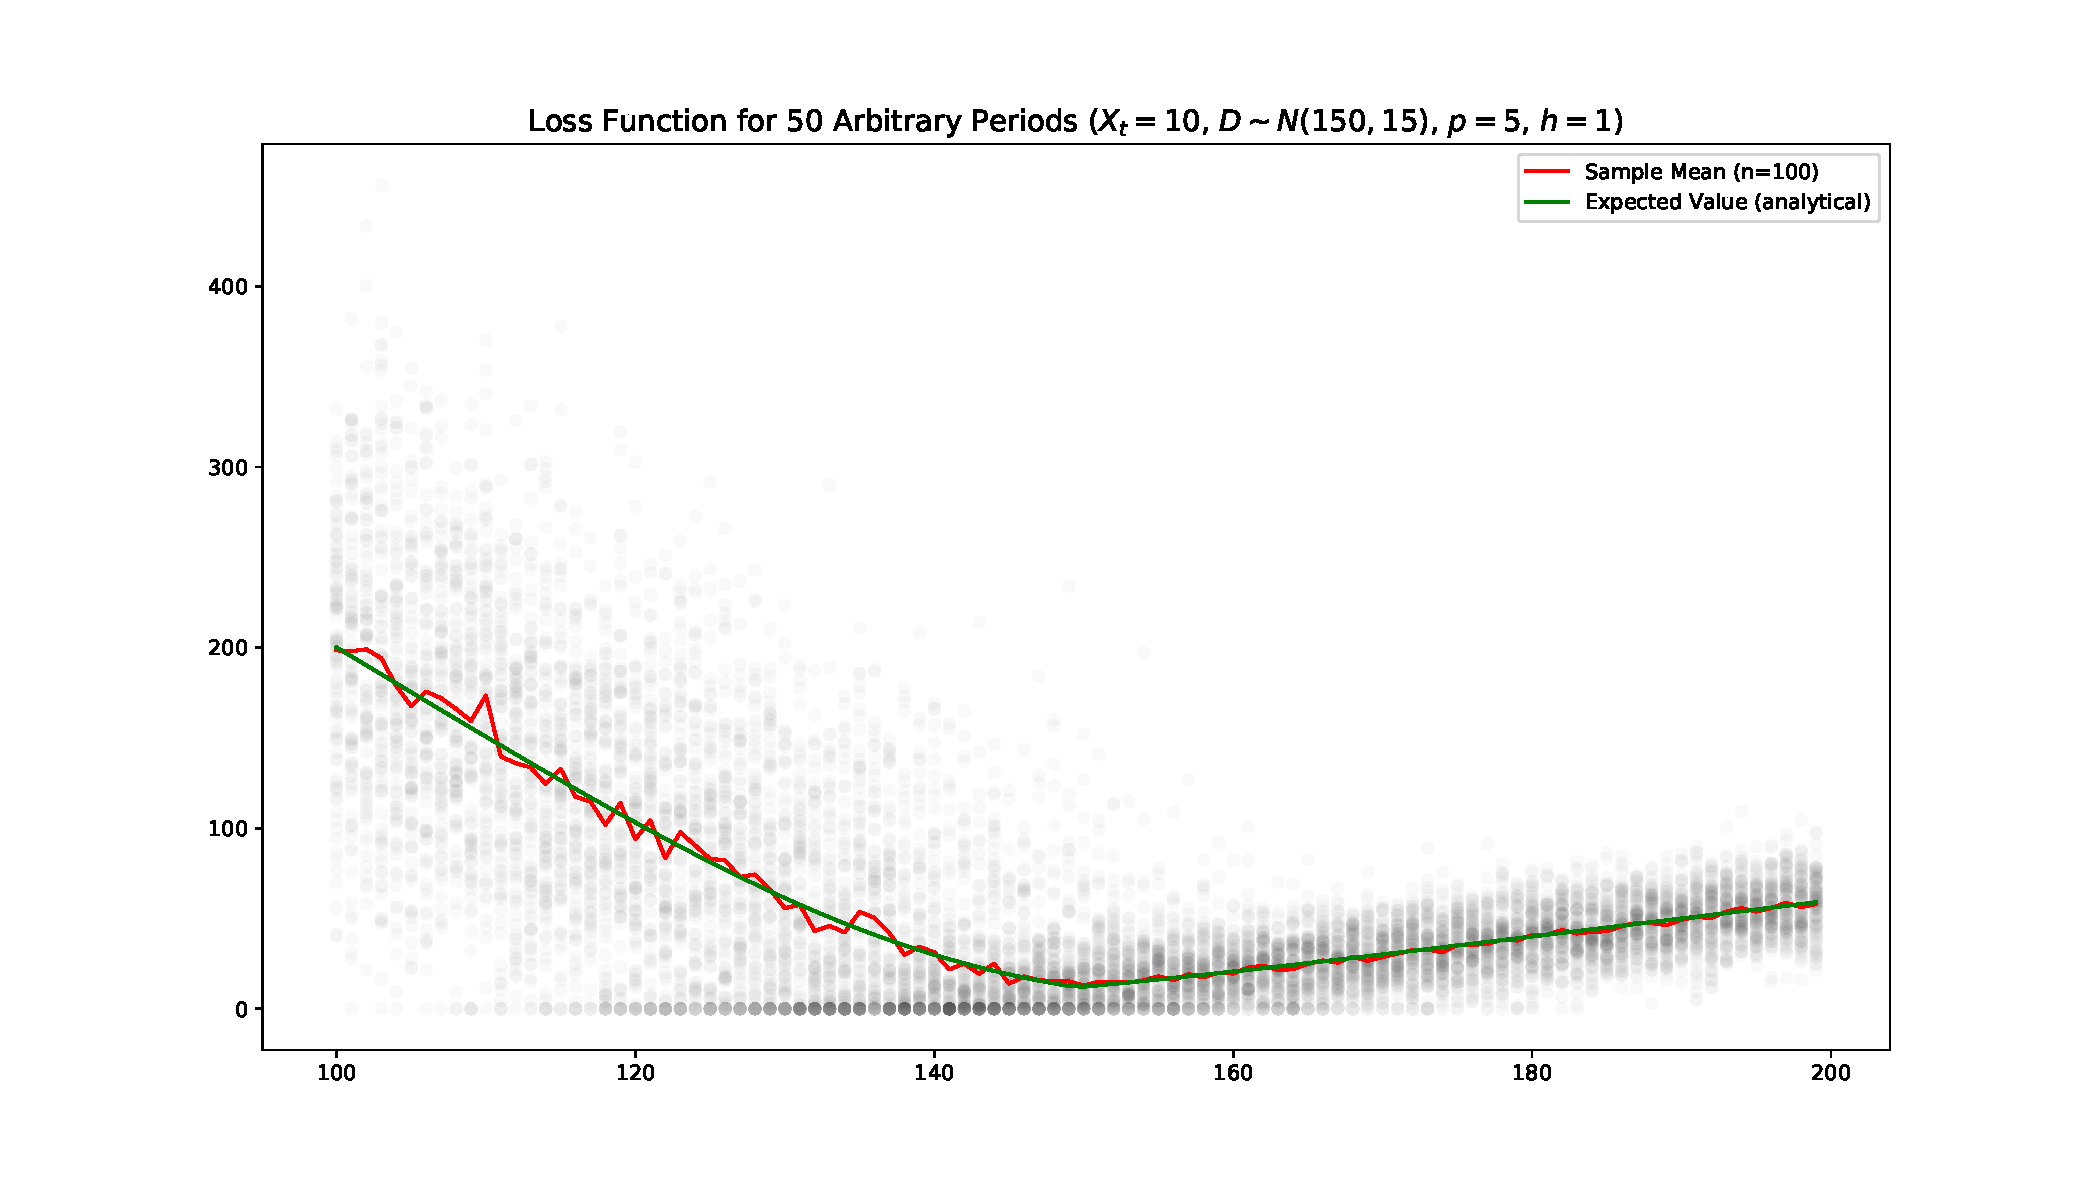
\includegraphics[width=\textwidth]{loss.pdf}

\section{Approximate Algorithms for Inventory Control}

When implementing these algorithms, I encountered many difficulties, particularly due to the intractability of one of the integrals resulting from the marginal cost accounting approach. Details on overcoming these difficulties are discussed in this section. 

\subsection{Dual Balancing Algorithm}

The Dual Balancing algorithm seeks the value $q_s^B$ such that: 
$$
	l_s^B(q_s^B) = \pi_s^B(q_s^B)
$$
Although there is an alternative convex minimization formulation, Levi et al suggests solving this in the root-finding formulation. The methods necessary to compute this root differ by the forecast type.

\subsubsection{Dual Balancing with Independent Forecasts}

Forecasting algorithms which provide independent forecast distributions allow for a more tractable solution. Practically speaking, this is a reasonable assumption: a large subset of forecasting algorithms (e.g. ARIMA variants) provide normally distributed forecasts. For this section we assume our forecasts are independently distributed. \\
\\
This would require locating the root of the following equation:
$$
	r_s^B(q_s^B) = l_s^B(q_s^B) - \pi_s^B(q_s^B) 
$$
Where the formulae for $l_s^B(q_s^B)$ and $\pi_s^B(q_s^B)$ can be found in equations (1) and (3). Levi et al suggests using the Bisection method (with linear convergence) to solve this. However, under our current assumptions, the derivative is available. This makes Newton-Raphson (with quadratic convergence) an option as well. The derivative for this equation is:
$$
	\frac{d}{dq_s^B} r_s^B(q_s^B) =  \frac{d}{d q_s} l_s^B(q_s) - \frac{d}{d q_s} \pi_s^B(q_s) 
$$
Where the formulae for $ \frac{d}{d q_s} l_s^B(q_s^B)$ and $ \frac{d}{d q_s} \pi_s^B(q_s^B)$ can be found in equations (2) and (4).\\
\\
Both Bisection and Newton-Raphson were tested for Scenario 1. The Bisection method required 49 evaluations of $r_s^B(q_s^B)$, while Newton-Raphson required 5 evalutions of both $r_s^B(q_s^B)$ and $\frac{d}{dq_s^B} r_s^B(q_s^B)$. The solved points $q_s^B$ differed by less than machine epsilon for both methods.

\subsubsection{Dual Balancing with General Forecasts}

For the general case, $l_s^B(q_s^B)$ cannot be computed without taking an integral over $T-s$ dimensions. This task cannot be done efficiently and accurately without some simulation approach (or more complicated procedures). \\
\\
To compute the root $q_s^B$, the Robbins-Monroe Algorithm was used. This requires the function $\hat{r}_s^B$, which evaluates $r_s^B$ for one demand sample, as well as an initial guess $q_s^0$. $q_s^B$ is then computed using the following equation:
$$
	q_s^i = q_s^{i-1} - \frac{1}{1 + i} \hat{r_s}^B(q_s^{i-1})
$$
This process can continue until convergence, or until some number of evalutations is reached. Because $q_s^i$ is not independent of $q_s^{i-1}$, it is generally useful to perform this process several times.\\
\\
Robbins-Monroe was used to recompute $q_s^B$ for the scenario discussed in the previous section. As shown in the plot below, convergence occurs within a few hundred iterations, and the final result is similar to the Newton-Raphson solution found previously. Because $\hat{r}_s^B$ is cheap to evaluate, the speed of this process is essentially limited by the random number generator. For this scenario, the Robbins-Monroe computing time was roughly an order of magnitude less than Newton-Raphson. 

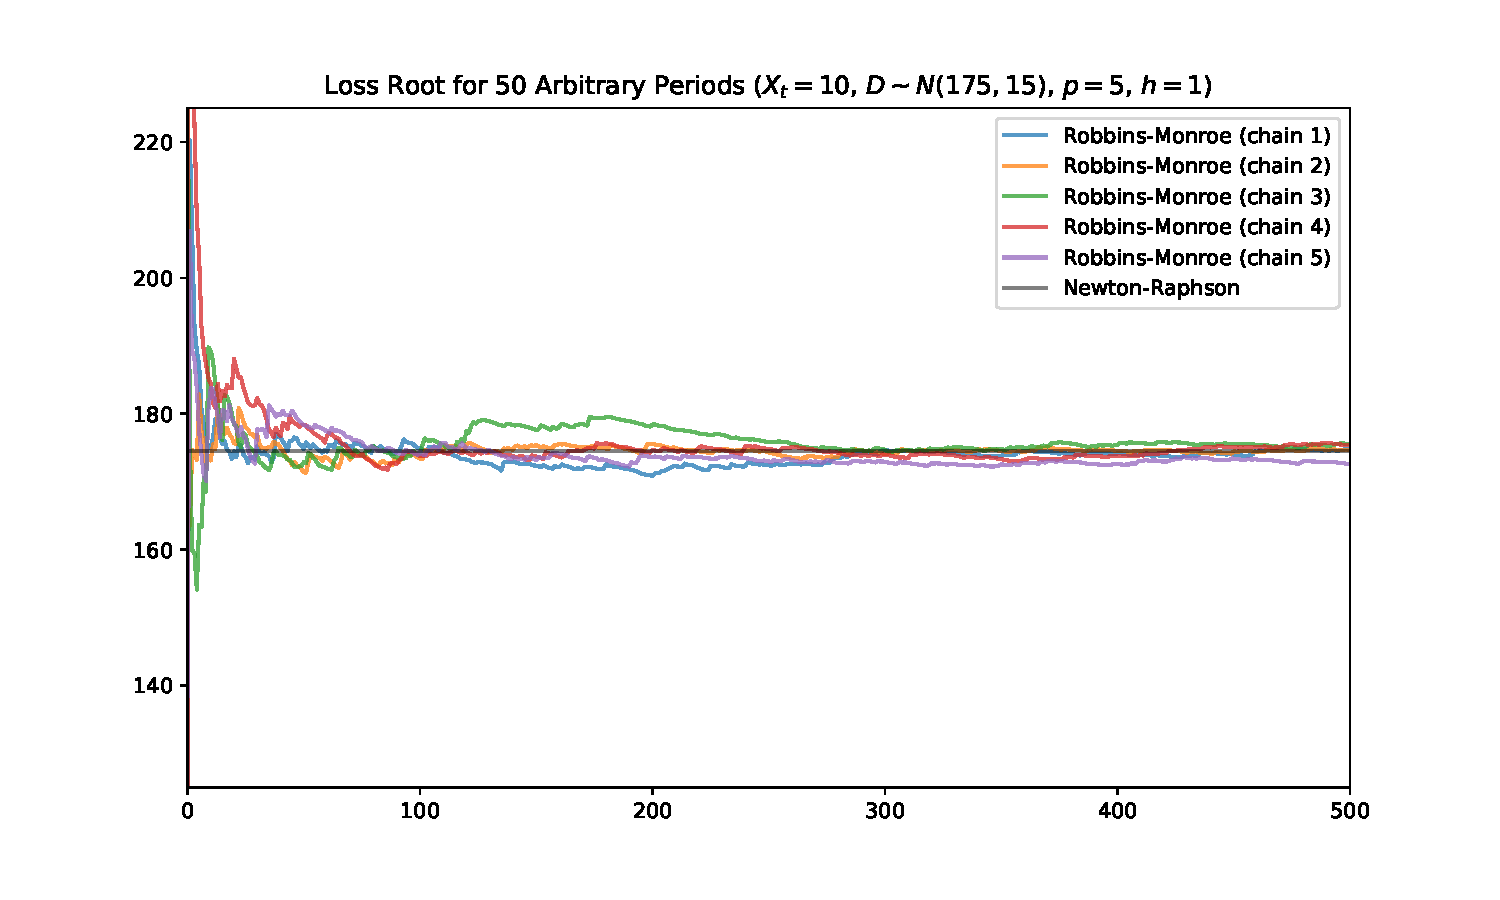
\includegraphics[width=\textwidth]{rbtraces}

\subsection{Triple Balancing Algorithm}

The Triple Balancing Algorithm seeks the value $q_s^B$ such that $q_s^B = \max\{q_s : l_s^B(q_s) \leq K\}$. This too is best viewed as a root-finding problem. As before, the computation needed to compute this will differ by the forecast type. 

\subsubsection{Triple Balancing Algorithm with Multivariate Normal Forecasts}

The approach taken here is similar to that of the Dual Balancing Algorithm. The root of the following equation must be located:
$$
	l_s^B(q_s) = K
$$ 
As above, there are some 
\end{document}